\documentclass [paper]{ieice}
\usepackage {cite}
\usepackage{graphicx}
	\graphicspath{{images/}}
\usepackage {latexsym}
\usepackage [varg]{txfonts}
\usepackage[none]{hyphenat}%%%%

\setcounter{page}{1}

%local definitions
\def\ClassFile{\texttt{ieice.cls}}
\newcommand{\PS}{{\scshape Post\-Script}}
\newcommand{\AmSLaTeX}{%
 $\mathcal A$\lower.4ex\hbox{$\!\mathcal M\!$}$\mathcal S$-\LaTeX}
\def\BibTeX{{\rmfamily B\kern-.05em
 \textsc{i\kern-.025em b}\kern-.08em
  T\kern-.1667em\lower.7ex\hbox{E}\kern-.125emX}}
\hyphenation{man-u-script}
\makeatletter
\def\tmpcite#1{\@ifundefined{b@#1}{\textbf{?}}{\csname b@#1\endcsname}}%
\makeatother
%end local definitions

\field{A}
\vol{01}
\no{01}

\title {Industry Application of Software Development Task Measurement System : TaskPit}
%\titlenote{This paper was presented at ...}

\authorlist{
 	\authorentry{Pawin Suthipornopas}{}{labelA}
 	\authorentry{Pattara Leelaprute}{}{labelA}
	\authorentry{Akito Monden}{}{}
	\authorentry{Hidetake Uwano}{}{}
	\authorentry{Yasutaka Kamei}{}{}
	\authorentry{Kenji Araki}{}{}
	\authorentry{Kingo Yamada}{}{}
	\authorentry{Ken-ichi Matsumoto}{}{labelB}
}
\affiliate[labelA]{Department of Computer Engineering, Kasetsart University}
\affiliate[labelB]{Nara Institute of Science and Technology}

\author{Pawin Suthipornopas,
		Pattara Leelaprute, \\
		Akito Monden, 
		Hidetake Uwano, 
		Yasutaka Kamei, \\
		Kenji Araki, 
		Kingo Yamada,t 
		Ken-ichi Matsumoto}
		
\date {2015-07-07}

\begin {document}

\maketitle
\begin {summary}
	To find any problems in a software development process, we have been developing an automated measurement tool called TaskPit, which monitors software development tasks such as programming, testing and documentation based on the execution history of software applications. This paper introduces the system requirements, design and implementation of TaskPit; then, presents two industry case studies applying TaskPit to actual software development. In the first case study, we applied TaskPit to 12 software developers in a certain software development division. As a result, several concerns (to be improved) have been revealed such as (a) a project leader spend too much time on development tasks while he was supposed to be a manager rather than a developer, (b) several developers rarely used e-mails while a company instructed developers to use e-mails as much as possible to leave communication records during development, and (c) several developers wrote too long e-mails to their customers. In the second case study, we have recorded the planned, actual, and declared time of development tasks. As a result, we found that (d) there were unplanned tasks in more than half of days, and (e) the declared time became closer day by day to the actual time measured by TaskPit. These suggest that TaskPit is useful not only for a project manager who is responsible to the process improvement but also for a developer who wants to improve by themself.
\end {summary}
	
\section {Introduction}
	
	To promote an idea of "Process Improvement via Measurement" in software industry, we had developed a software development task measurement system called TaskPit\cite{taskpit} in 2008, and have been updating it till today. TaskPit automatically records the time and the amount of work of daily tasks of an individual developer or a development team to find any problems in software development. It can record the time spent for each task such as "Programming" using Eclipse or Visual Studio, "Documentation" using Word or other text editors, "E-mail" using Gmail on a browser and so on, where a task is associated with a set of applications and window titles. TaskPit records an amount of work for each task in terms of the number of keystrokes and the mouse clicks. It can also records an amount of deliverables of each task as the increased size of files in a directory associated to the task. \par
	To date, the TaskPit community has been gradually grown up, user manuals and related tools have been developed by volunteers, and as of July 2015, total downloads of TaskPit version 1.0.0 to 1.0.3 has reached 1500\cite{taskpit}. Now we are demanding for industry case studies to share the experience and findings about how TaskPit could be used for process improvement. \par
	This paper introduces the system requirements, design and implementation of TaskPit; then presents industry case studies applying TaskPit to two software organizations. The first organization consists of 12 members, measured in 9 days (6 business days) where 7 are developers, 3 leaders, and 2 customer services. Analysis of data and measurements of the work surveyed in departments are collected and summarize by one veteran employee from other department to look after the flow of their work. In the second organization there is only one developer measured in 17 days (13 business days) measured by TaskPit. In addition to the automatic measurement TaskPit did, there is also a value plan and engage time for each development tasks for this developer each day. This is to clarify the difference between the measured value that was collected and analyze manually, and automatic measurement. \par
	Please note that this paper is an extension of our Japanese workshop paper (short paper) [FOSE2013] with an additional (second) case study. In this paper we also added explanations of the system requirements, design and implementation of TaskPit to clarify the design concept of TaskPit and to illustrate how TaskPit can be used in software organizations. \par
	In the following Chapter 2, we will describe the related work and research in background, Chapter 3 will be about TaskPit and its system requirements, design, and implementation. In Chapter 4 and 5 will be measurement results and analysis in two organizations. Lastly in Chapter 6 is a summary.
	
\section {Background and Related Work}
	
	As Tom DeMarco said 「You can't control what you can't measure」we believe it is essential to control the process of developing software\cite{demarco1986controlling}. For this purpose, various product processes metrics and measurement have been applied to the developing site\cite{grady1992practical}. In many of the environment of development site; the software scale, work hours, and bugs are measured and used for project management, and quality assurance of the development\cite{nec2010software}\cite{putnam2013five}. \par
	On the other hand, problems found in the development field are mostly from human factors\cite{sec2010itproject} rather than the product process and measurements. This is considered to be natural as described in Personal Software Process (PSP) and Team Software Process (TSP), where developers and the development team follow up the work of day-to-day tasks and record everything manually, these methods are well-known as a method for process improvement\cite{humphrey1995discipline}\cite{humphrey2001}. However, as developers have to do this manually, this method popularity grows thin and does not spread widely as it should. \par
	At first, PSP has been proposed as a measurement procedure in accordance with a specific measurement form which required accurate calculation and required great cost to the data measurement. There are also tools and systems that act as a supporting role in data measurement to help calculating data more easily such as Process Dashboard\cite{processdashboard}, Task Coach\cite{taskcoach} and Slim Timer\cite{slimtimer}, but using these tools will required to switch the measurement work (Context Switching) because they are all in different environment, and this has become a barrier in introducing the measurement procedure to the development site\cite{sillitti2003collecting}. \par
	Without causing the Context Switch, automatic measurement tools on software development have been proposed, for example EPM\cite{ohira2004empirical}, Ginger\cite{}, Ginger2\cite{torii1999ginger2}, HackyStat\cite{}, and PROM\cite{}. Detailed data collected by these tools can be used with less cost. \par
	In this paper, the main objective is to support the introduction of process improvement in the development team. It is easy to introduce TaskPit as a system that does not require pre-planning, and capable of carrying out process improvement through measurement. TaskPit will record the number of hours and amount of work separately task by task, and can automatically measure the changes in the result number compared to actual number. Data in the system is to measure the amount of work, and achievement in each task are directly represents and are easily analyzed. It is suitable for the stage of process improvement during development.
	
\section{TaskPit}

\subsection{System Requirements}
	Based on the previous chapter of this paper and the requirements of task measuring system, our system requirements are described in detail in the following subsection: \par
	
\subsubsection{[Requirement 1: Binding between Tasks and Applications]}
	In TaskPit system, each development task are to be work on different applications and windows. Therefore, we need to bind the task name with application name corresponding to it (the executable file name or process name). However, in the actual work, it is not always necessary to use only one application to perform one task. One application might work on many tasks, and one task might be completed by many applications. Moreover, even in different tasks, it may use the same application. In such a case, to distinguish tasks by differences in the character string in the name of the window during application execution, we approach it with BNF as follows: \par

\begin{itemize}
	\item[] $\langle$Task$\rangle$ ::= $\langle$Application$\rangle$ \{$\|$$\langle$ Application $\rangle$\}
	\item[] $\langle$Application$\rangle$ ::= $\langle$Executable File Name$\rangle$ [$\langle$Window Name$\rangle$]
\end{itemize}

	Tasks are defined as a set of one or more running applications, and applications are defined as a set of executable name and window name. Below are examples of how tasks are defined. \par
	
\begin{itemize}
	\item Mail = OUTLOOK.EXE $\|$ IEXPLORE.EXE "Gmail" $\|$ CHROME.EXE "Gmail"
	\item Documentation = WINWORD.EXE $\|$ NOTEPAD.EXE $\|$ TERAPAD.EXE
	\item Browsing = IEXPLORE.EXE $\|$ CHROME.EXE
	\item Searching = IEXPLORE.EXE "Google" \newline $\|$ CHROME.EXE "Google"
	\item Spreadsheet = EXCEL.EXE
	\item Programming = eclipse.exe $\|$ devenv.exe
	\item Testing = mstsc.exe $\|$ Beyond32.exe $\|$ DF.exe
\end{itemize}

\subsubsection{[Requirement 2: Automated Data Measurement]}

\noindent $\bullet$ Task Execution Time Measurement \par
	Time will start recording for each of the application and window when "Application is in use" which refers to a state where that window is currently in focus. However, even if it is in focus, if the time has passed (10 minutes) without active computer input (mouse and keyboard), it will be recorded as not using any application. \newline

\noindent $\bullet$ Amount of Work Measurement \par
	Amount of work will be recorded by the input of the computer, refers to keyboard strokes and mouse clicks. \newline
	
\noindent $\bullet$ Files Measurement \par
	For each task file, it will be defined as a directory and file extensions. TaskPit scans the files under specified directory and measure the increasing  and decreasing number of total file size and number of files in intervals. The definition is described below in BNF.

\begin{itemize}
	\item[] $\langle$Artifact$\rangle$ ::= $\langle$Directory$\rangle$ $\langle$Extension$\rangle$ \{$\langle$ Extension $\rangle$\}
\end{itemize}

\noindent And below are some examples. \par
	
\begin{itemize}
	\item[] Requirement analysis documents = 
	\item[] "C:$\backslash$Users$\backslash$monden$\backslash$desktop$\backslash$development$\backslash$SRS", 
	\item[]"doc,tex,txt"
	\item[]Design documents = 
	\item[] "C:\textbackslash Documents and Settings\textbackslash monden\textbackslash desktop\textbackslash 
	\item[] development\textbackslash sources", "c,cpp,java" \newline
\end{itemize}

\noindent $\bullet$ Regarding Privacy \par
		During the measuring process of the team, it is necessary to protect personal information and keeping the privacy of developers in a comfort zone. In the proposed system, application name, windows name, file name, and many more are not recorded to prevent the feeling of being "monitored" by the user, because it could cause negative feedback to the system we introduced. Any other window or application that user open up will instead recorded as "Other Tasks".
		
\subsubsection{[Requirement 3: Team measurement]}
	Data measured for each user is collected at one time with timestamp placed with each task in the team unit, and then count up amount of efforts and products produced.
	
\subsubsection{[Requirement 4: Data visualization]}
	To visualize the measurement results in the development team, for a specific period of time we can display the graph as a bar chart or line chart to visulize total time spent doing tasks and total time spent during work by using timestamp from the result log file of our proposed system. The data visualization will require a log file from proposed system, compiled it into a pre-processed version to sum up all work hour and visualize in graphics. ***Will add charts that can visualize keystrokes and mouse clicks in the future*** Chart of total time spent on tasks and total work hour will look like Figure \ref{fig1} and Figure \ref{fig2} respectively.
	
\begin{figure}[h]
	\centering	
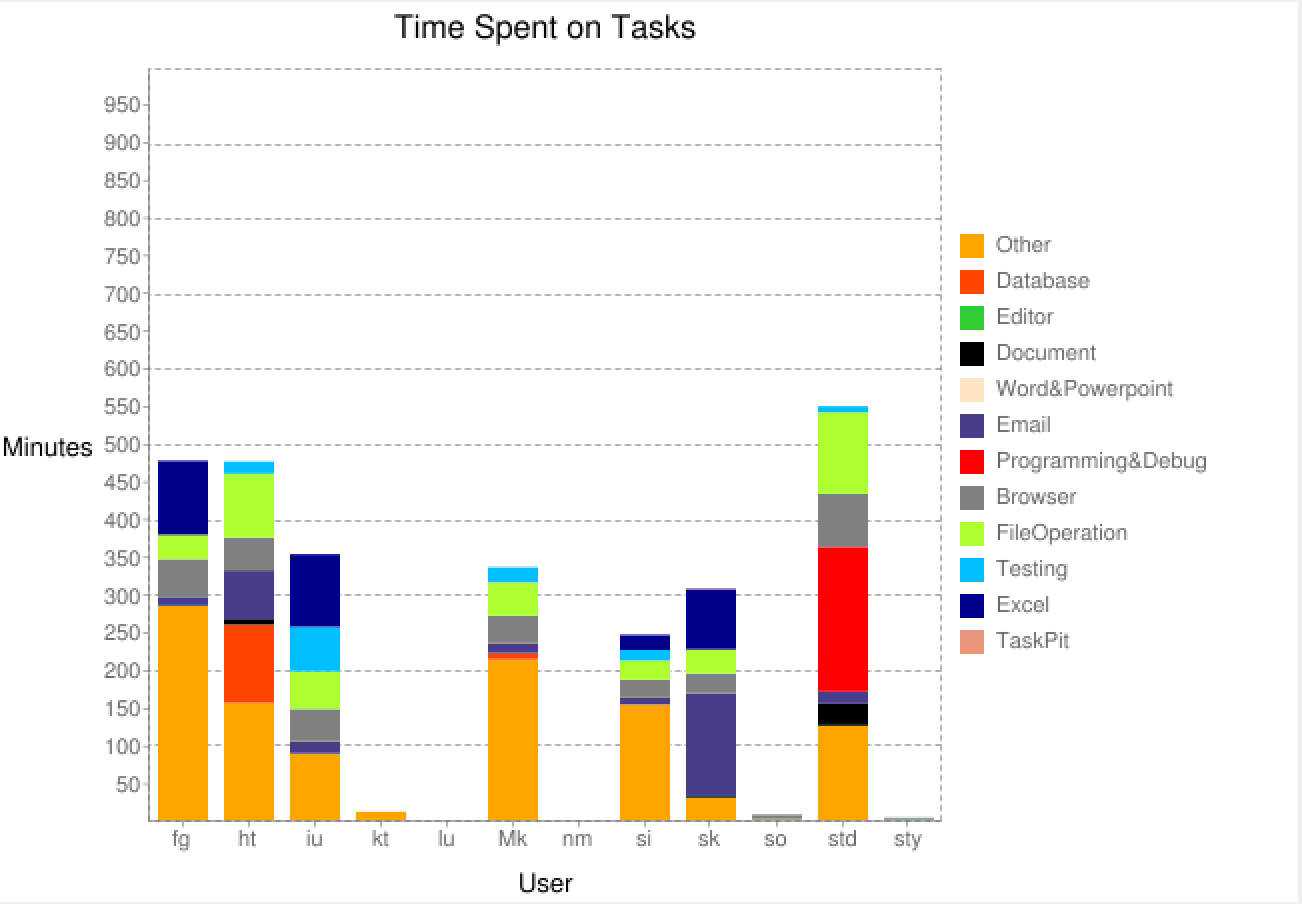
\includegraphics[width=0.5\textwidth]{fig1}
	\caption{Total time spent on tasks}
	\label{fig1}
\end{figure}

\begin{figure}[h]
	\centering	
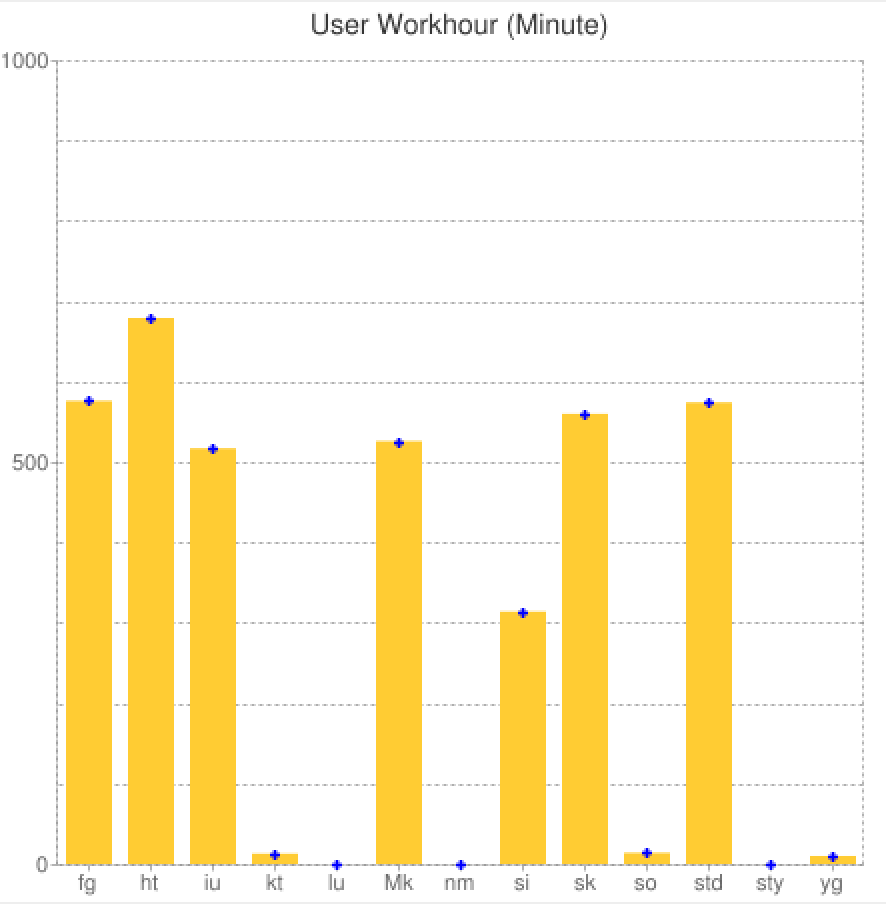
\includegraphics[width=0.4\textwidth]{fig2}
	\caption{Total work hour}
	\label{fig2}
\end{figure}

\begin{figure}[h]
	\centering	
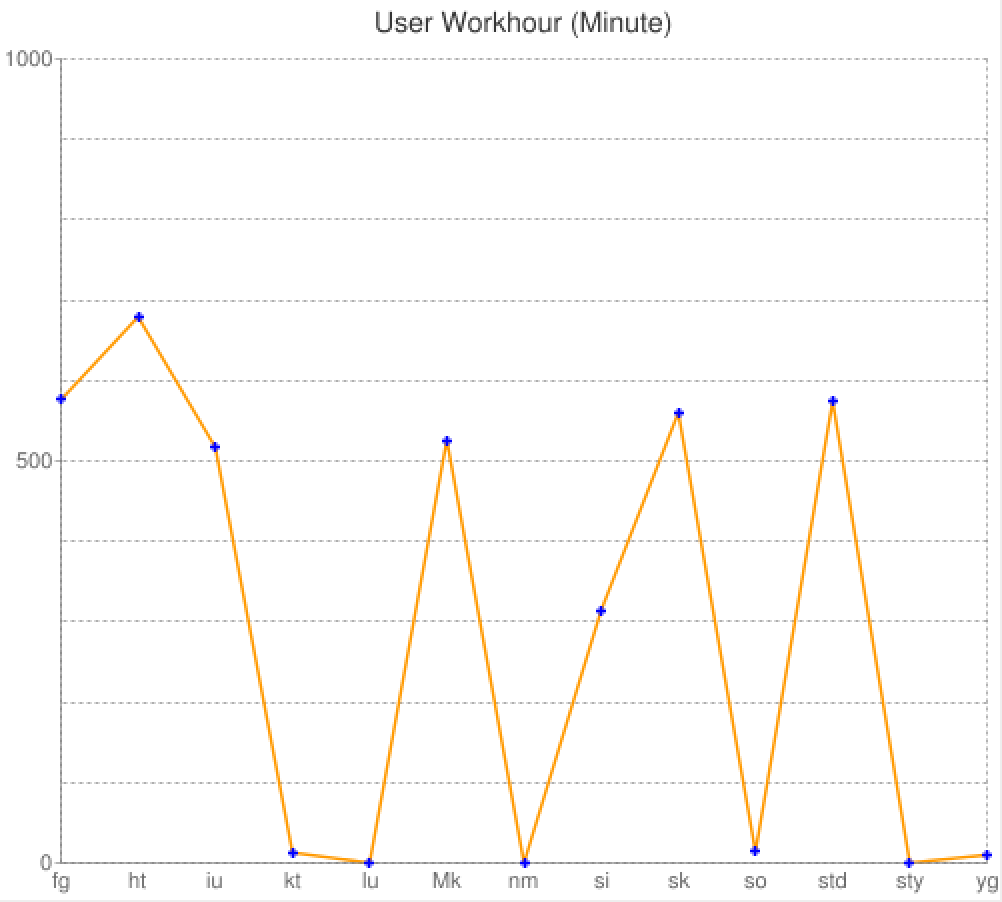
\includegraphics[width=0.4\textwidth]{fig3}
	\caption{Total work hour in Line Chart}
	\label{fig3}
\end{figure}
	
\subsection{System Design}
	As shown in Figure \ref{fig4}, TaskPit have its own database working at the back end of the system along with the visualization unit, configuration, and log files with daily report. In the configuration file will contain definitions of task and file as described before in the requirement section to be able to generate output of time interval of usage of each task and program in the log file. In Figure \ref{fig5} is the user interface of the program. Each task will record its own execution time by accumulating all time it has been in focus along with number of keystrokes and mouse clicks. \par
	To meet up the requirement of being less burden to the overall system and without providing server too much load, there will be a specified shared directory to store measurement result. Visualization tool is also used with configuration files and log files to graph visualize chart from various aspects of measurement results for specific period of time. Working in the client to server fashion as shown in Figure \ref{fig6}. \par
	In addition, an overview report of daily work can be generated in both CSV format and in Excel .xls format. \par
	
\subsection{Implementation}
	TaskPit 1.0.X operates using .Net Framework on  Windows XP, Vista, and 7. Database requires SQLite and tasks are performed using Windows API. To handle the current active windows we invoke GetForegroundWindow, window title is obtained using GetWindowText. To get process we use GetProcessById method with System.Diagnostics.Process class to obtain execution file name. \par
	Similar to tasks, the keystrokes and mouse clicks is measured by registering a method to hook the keyboard and mouse events in SetWindowsHookEx. In addition we also measure files with GetFiles method from System.IO.Directory class at regular time intervals to scan the files specified in that directory to measure number of files and file size. \par
	Once everything has been recorded and done in one interval of choice, whether days or weeks, it will generate CSV file as an output. This CSV file is the log of everyone measurement which will be used to compile into one work hour sheet and another pre-processed data log file sheet required to visualize a graph of total time spent in tasks and total work hour of every developers by using Google Chart API and a framework called charts4j to run Google Chart API using Java language.
	
\section{Case Study 1: Team Measurement}

\subsection{Goal of Measurement}
	In the first case study in one software development organization, we believed that to discover the clues of problems in the development department will lead to improvements, so to carry out the analysis of measurement results, we assign one veteran employee as a manager and support department which function as a Project Management Office (PMO). This person will act to make sure of quality control and standards of enterprise-wide project from the point of view of human, and in terms of assistance of consulting, this analyst has to grasp the role of each team members, which he or she did not know until the beginning of the work.
	
\begin{figure}[h]
	\centering	
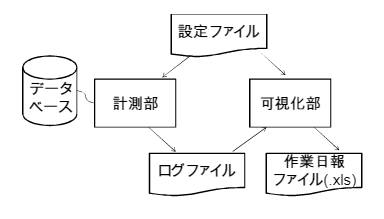
\includegraphics[width=0.5\textwidth]{fig4}
	\caption{Overall System}
	\label{fig4}
\end{figure}

\begin{figure}[h]
	\centering	
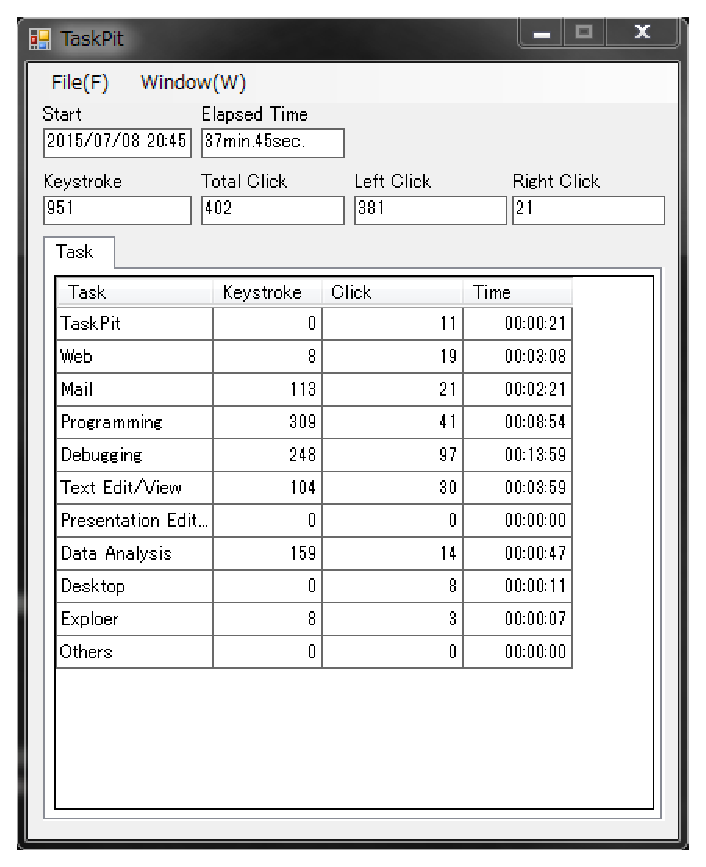
\includegraphics[width=0.4\textwidth]{fig5}
	\caption{TaskPit User Interface}
	\label{fig5}
\end{figure}

\begin{figure}[h]
	\centering	
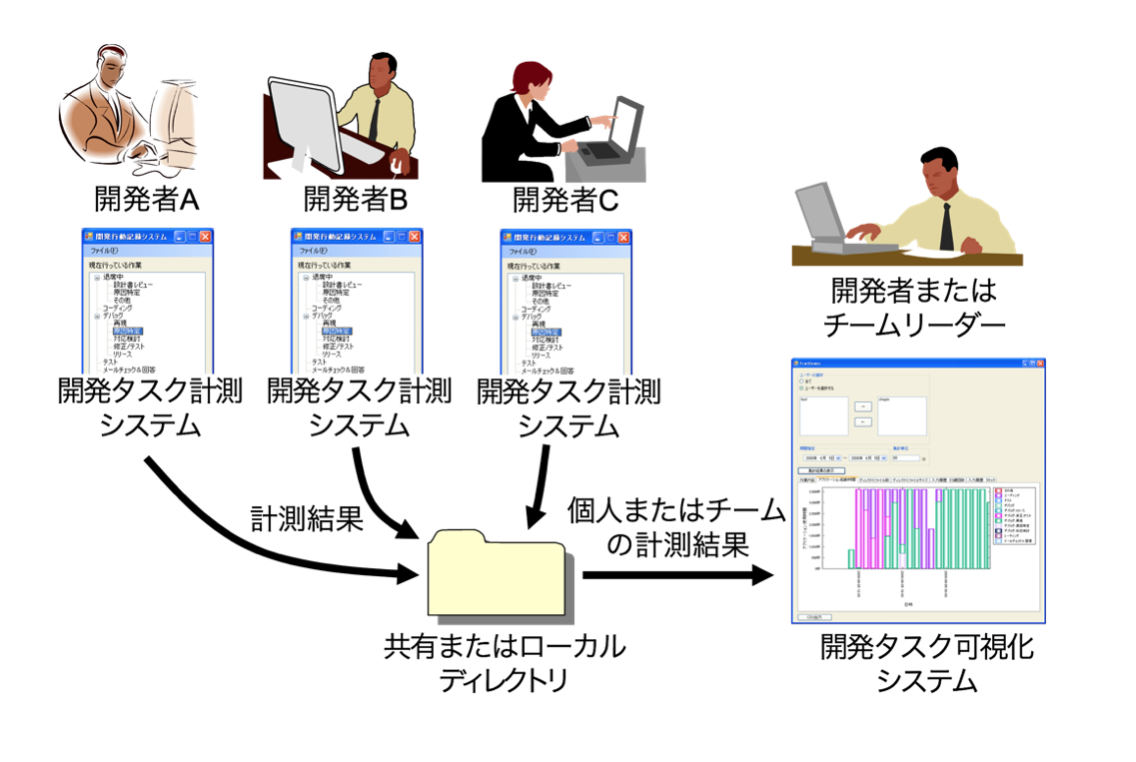
\includegraphics[width=0.5\textwidth]{fig6}
	\caption{Shared System}
	\label{fig6}
\end{figure}
	
\subsection{Measurement Target and Time}
	The target of the measurement is the department of software development consists of 12 people in total. As shown in Figure.\ref{fig7}, each person's role in the department are different. With 3 main leaders, 3 developers in Project A, 4 developers in Project B, and lastly with 2 customer supports. Project A is really busy since the deadline of the project is very near, while Project B is more relaxed since the deadline is further away. Member B1 of the Project B is not familiar with the environment since that person has recently been moved from other department to this department in one month. In addition, 2 customer supports (CS1, CS2) has shorter working hour than what was planned. \par
	In this department we used Trac as a project management tool for the browser, which has been encouraged to carry out material management and communications. In data measurement we used TaskPit 1.0.1 with modified components to hide GUI from the user to prevent disturbance during work. We also did some interviews for applications used in this department to link up the program with TaskPit. Measurements were carried out over for total of 9 days (6 business days).

\begin{figure}[h]
	\centering	
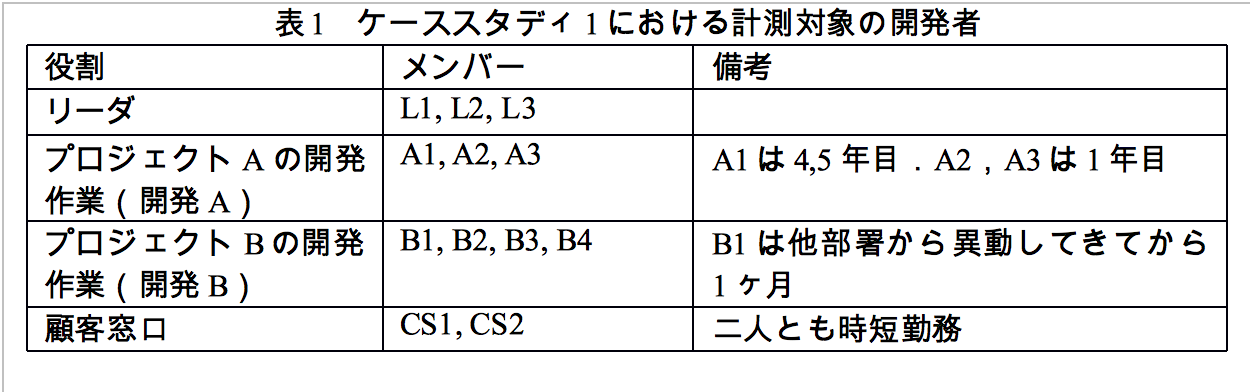
\includegraphics[width=0.5\textwidth]{fig7}
	\caption{Team Roles}
	\label{fig7}
\end{figure}

\subsection{File Configuration}
	As shown in Figure \ref{fig8}, file configuration is done by assigning multiple applications to a task.
	
\begin{figure}[h]
	\centering	
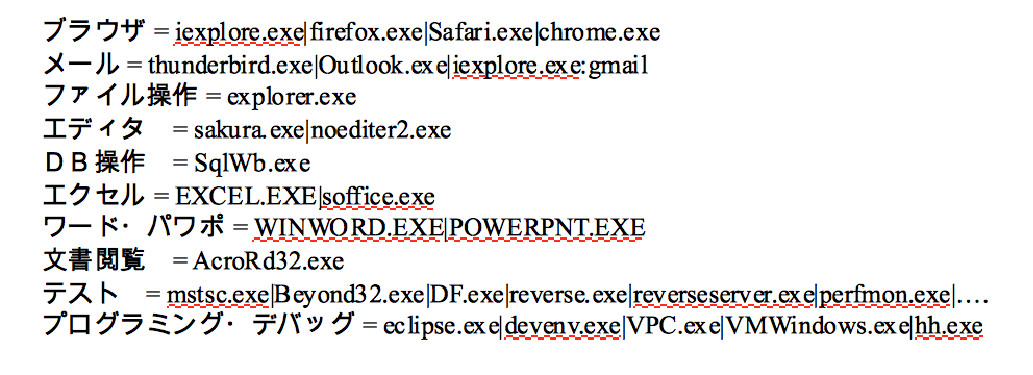
\includegraphics[width=0.5\textwidth]{fig8}
	\caption{File Configuration}
	\label{fig8}
\end{figure}

\subsection{Measurement Results and Analysis}
	From Figure \ref{fig9} is time spent in each tasks, shows a working time of respective mean value per day. Working hours are collected from the start to the end of using TaskPit. The obtained results are as follows.\par
	
\begin{figure}[h]
	\centering	
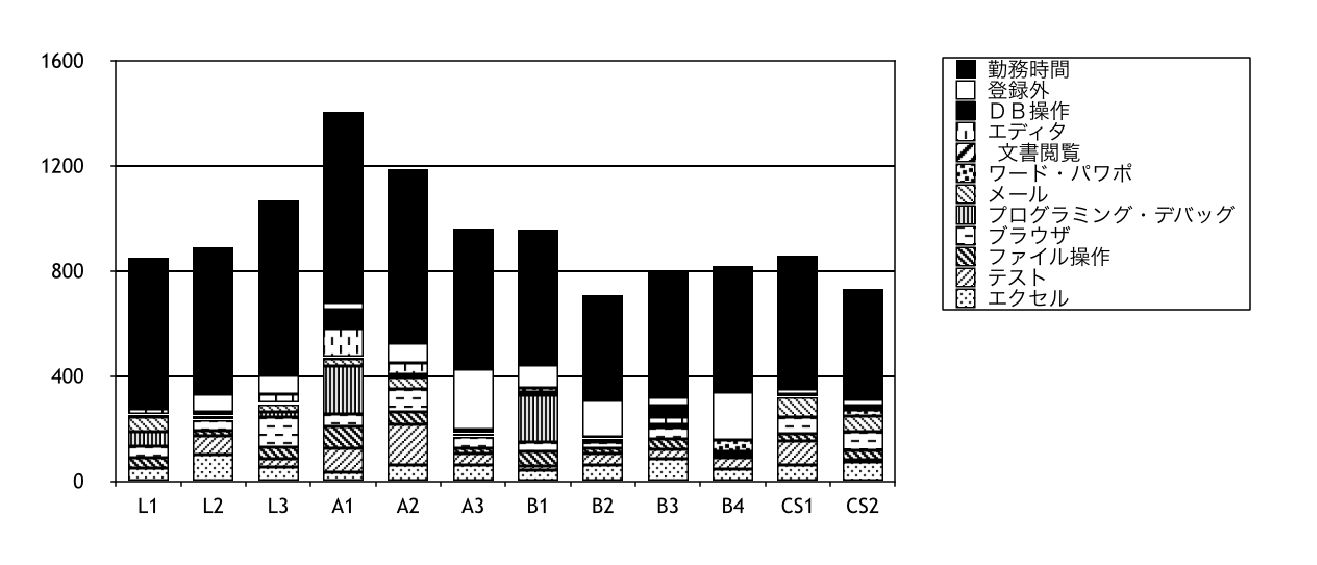
\includegraphics[width=0.5\textwidth]{fig9}
	\caption{Time Spent}
	\label{fig9}
\end{figure}

\begin{itemize}
	\item As shown in Figure \ref{fig9} there are tasks that were unregistered in every developers. With A3, B2, B4 in particular who exceeded 100 minutes in this category. One of the cause of this for this department is because new program and unidentified application can be installed into this pre-determined application only PC. There is a case where unspecified application is detected. Also the attendance management system for the developers was not registered in the configuration file. Furthermore, TaskPit can not measure testing or debugging that happens in Virtual OS. (This was fixed in TaskPit 1.0.3 so that Virtual OS can be measured normally)
	\item Overall working hours of members in Project A (A1, A2, A3) is longer. Project A is also closer to the deadline with members working hours really close to the time they were given. On the other hand B1, B2, B3 and B4 are progressing steadily with shorter work hours compared to Project A. By the work of TaskPit, it can be concluded that this program can grasp a hold of how busy a project is.
	\item Person with the best performance is A1, as seen from the PC work time and actual work hour are really close together. Spent 184 minutes debugging, 106 minutes editing and another 94 minutes testing. A1 is definitely a programmer who actually work on the task given. Meanwhile, A2 who belongs to the same project spent 0 minute debugging (with unregistered 76 minutes to be added), along with 156 minutes testing. TaskPit is able to understand the work of each developer by visualizing it.
	\item The relationship between working hours and work time on PC is shown in Figure \ref{fig10}. From this figure, leaders spent little time in PC compare to working hours than those of developers and customer support. This is due to the leaders having to spent time working in business and management part rather than developing and coding. However, leader L2 has slightly larger PC time compare to other leaders. Breaking down the tasks, leader L2 had engaged on average 71 minutes in testing along with 103 minutes in excel program operation. As a leader this could be said that too much time is spent on development work.
	\item Two customer supports (CS1, CS2) as seen on the chart are mostly engaged into mailing and browsing. This is due to their work requires communicating and interacting with customers via e-mail. It is suggests that we apply material management using Trac on the browser. (In this measurement, the problem of not being able to reflect differences in tasks on the browser configuration is also revealed here.)
	\item Looking at mail tasks, L2, A3, B1, B2, B3, B4 are all spent less than 15 minutes here. In this department we have encouraged members to use e-mail more than telephone as a communication method (in order to keep the record for later). From this fact, it can be said that L2 has spent too little time using e-mail, and furthermore L2 has been reported with more extensive use of telephone.
	\item Figure \ref{fig11} shows time spent in mailing and programming along with their respective typing speed (or key strokes). Comparing key strokes per minute for the e-mail tasks, CS1 and CS2 seems higher. It could be possible that the content in e-mails of these members are longer or could be the cause of typing correction. The mail exchanging with customer requires simplicity and quality in terms of information along with descriptive content. It is possible that we could use an improvement in mail writing.
	\item Looking from Figure \ref{fig11}. It is possible that A1 is the most productive, excluding quality, among other member of this team, as told by his typing speed is rather high along with his over-the-top time spent in programming and debug.
\end{itemize}

\begin{figure}[h]
	\centering	
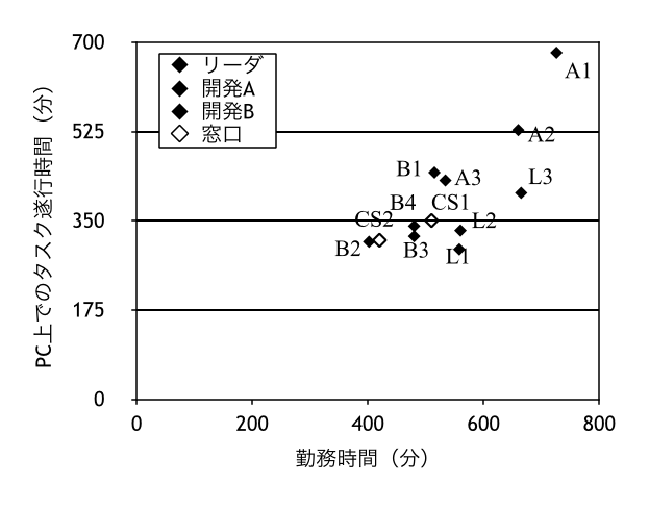
\includegraphics[width=0.5\textwidth]{fig10}
	\caption{PC Work Time and Working Hour Relationship}
	\label{fig10}
\end{figure}

\begin{figure}[h]
	\centering	
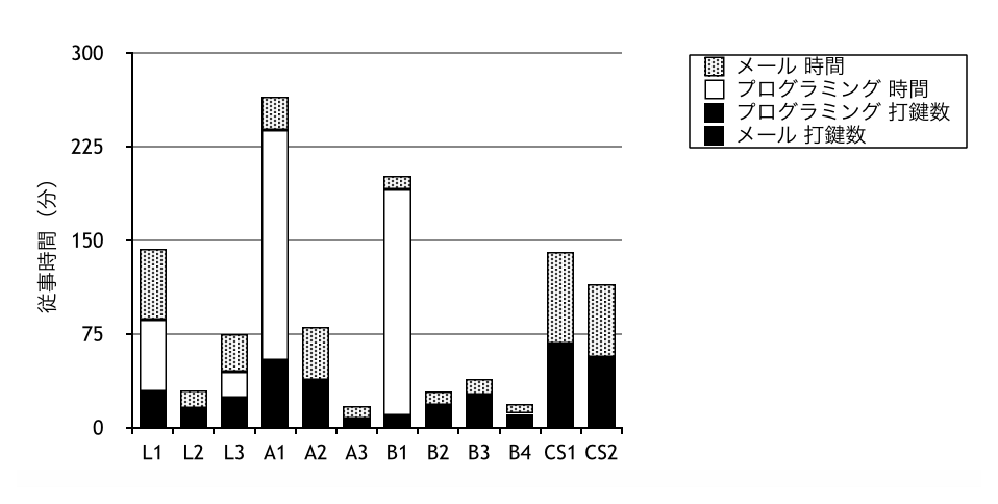
\includegraphics[width=0.5\textwidth]{fig11}
	\caption{Mail and Programming}
	\label{fig11}
\end{figure}

\section{Case Study 2: Personal Measurement}

\subsection{Measurement Purpose and Methods}
	In this second case study, the developer performed his own measurement and analysis assuming that it would lead to self improvements. The developer will set his own planned value for each development tasks for everyday and also measure value everyday to see the difference. Planned value is the value developers set at the beginning of the day to be a goal. The measured value is value obtained by TaskPit. The developer will also report his own measured value at the end of the day before comparing with TaskPit.\par
	If the value of planned and measured are close together, even without using TaskPit, that developer is able to perform tasks along what was planned and has responsibility in his given work. However, if large difference between measured and reported value are presented, the developer may not be able to understand the implementation time of the task. Also when there are large difference between what was planned and what was measured, this is a serious problem as you can not manage your time well.

\subsection{Measurement Target and Period}
	The target of this measurement belongs to a different organization from the first case study. The web-based programming developer who was tasked for total 17 days (13 business days). Prior to this measurement, the developer studied and learnt the configuration file of TaskPit in 3 days. Also at the end of the daily work, planned values and measured values are asked to be presented and to give comments upon them.

\subsection{Measurement Results and Analysis}
	Measured value and planned value are shown in Figure \ref{fig12} and Figure \ref{fig13} respectively. The horizontal axis of each graph is the number of days and the vertical represents number of hours. Measured values are likely to be smaller than what is planned, except for day 11. From the comment presented by the developer, this is because he did not use the personal computer on day 4, while first three days is because of unexpected amount of work. In fact, the unplanned work was planned to be included from the start by the amount of 5 to 10 percent of total work, revealed by TaskPit. This should be noted however, that the planned value up to the day 11 was intended to be like what figures have shown.
	In Figure \ref{fig14} shows the subtraction of measured value from the planned value. As shown in the figure, as time passed working on a task using TaskPit in the process, the time estimated has become closer to the actual measured value. Therefore in this case, by continuously usage of TaskPit, one can assume that developers can understand their workload correctly. "Working is now easier and now planning time and actual time are much closer together.". Therefore, by using TaskPit, developers are now aware of actual time and planned time and can develop themselves to exceed the expectation of what is planned. It is expected that this could be of use in managing and planning in development works. 

\begin{figure}[h]
	\centering	
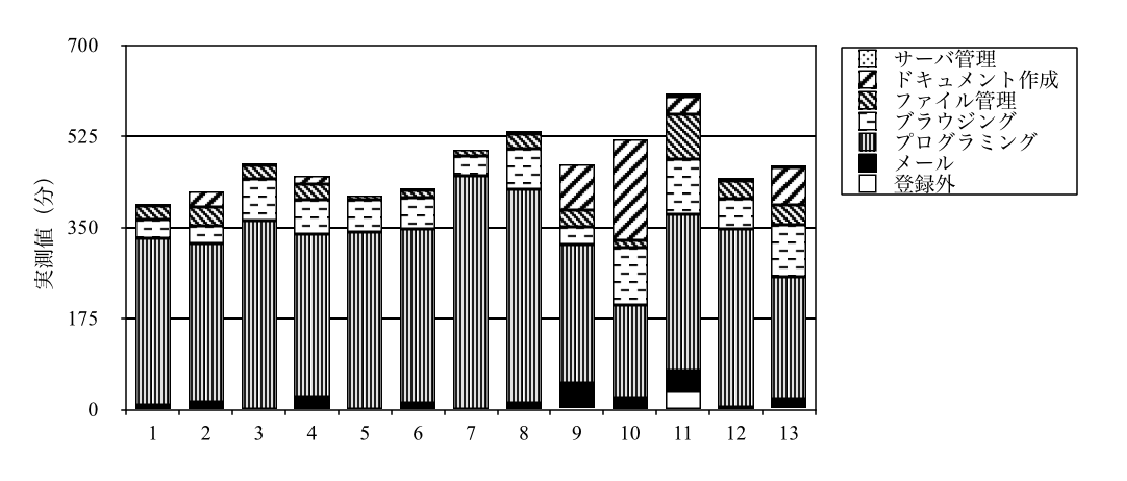
\includegraphics[width=0.5\textwidth]{fig12}
	\caption{Measured Value}
	\label{fig12}
\end{figure}

\begin{figure}[h]
	\centering	
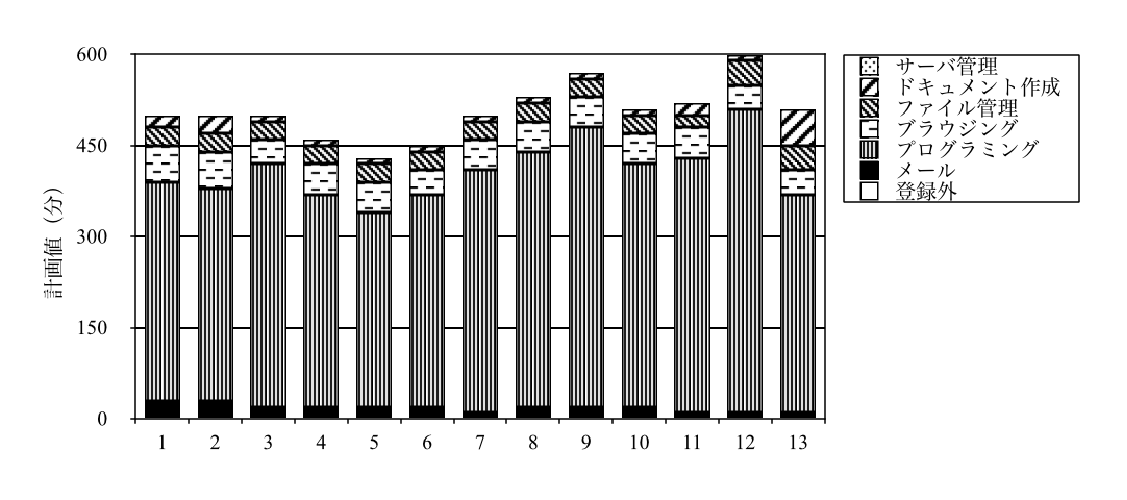
\includegraphics[width=0.5\textwidth]{fig13}
	\caption{Planned Value}
	\label{fig13}
\end{figure}

\begin{figure}[h]
	\centering	
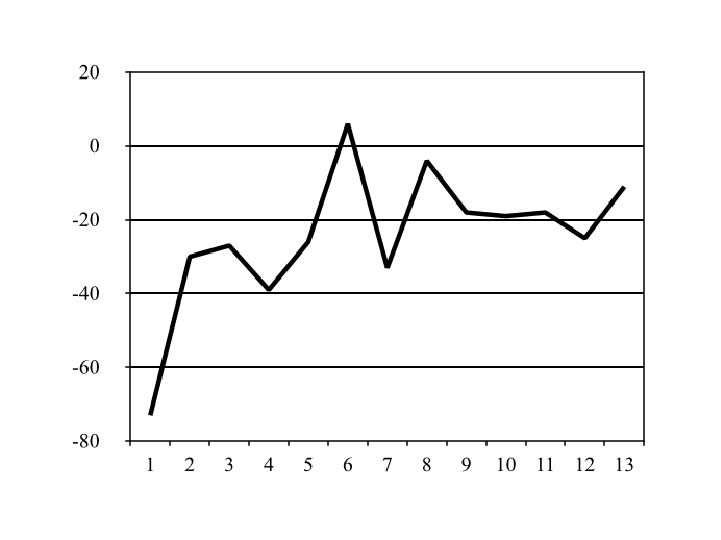
\includegraphics[width=0.5\textwidth]{fig14}
	\caption{Result Value}
	\label{fig14}
\end{figure}

\section{Summary}
	In this paper, we clarified the effect of the automatic measurement in software development work for the purpose of publishing its findings and to apply it with two development organization. The first one was to measure 12 developers over six business days. It was found that it is possible that TaskPit can grasp and explain how busy the development process and each project of each developers are. In addition, it is estimated that (a) leader spent too much time developing, and not many people are communicating through e-mail. (b) In contact with customers through the e-mail, the content inside these mails are too long and was addressed in short period of time. Lastly (c) there is a possibility that there could be a room for some improvements in e-mail writing.
	In the second organization, we observe and measure the developer who is tasked on developing web-software for 13 business days and recorded all measured and planned values. As a result (d) unplanned work was found more than half of the total work in a day, but (e) in the end the total work hours obtained from the measured data exceeds the expectation of what is planned, by using TaskPit to help managing and understanding developer's own work.
	With more case studies and findings in the future, we expected this project to help many organizations in development process. The authors will continue working on application cases of TaskPit and expected to continue publish newly obtained findings.

\bibliography {taskpit}
\bibliographystyle {plain}
	
\end {document}